\documentclass{article}
\usepackage[utf8x]{inputenc}
\usepackage{ucs}
\usepackage{amsmath} 
\usepackage{amsfonts}
\usepackage{marvosym}
\usepackage{wasysym}
\usepackage{upgreek}
\usepackage[english,russian]{babel}
\usepackage{graphicx}
\usepackage{float}
\usepackage{textcomp}
\usepackage{hyperref}
\usepackage{geometry}
  \geometry{left=2cm}
  \geometry{right=1.5cm}
  \geometry{top=1cm}
  \geometry{bottom=2cm}
\usepackage{tikz}
\usepackage{ccaption}
\usepackage{multicol}

\hypersetup{
   colorlinks=true,
   citecolor=blue,
   linkcolor=black,
   urlcolor=blue
}

\usepackage{listings}
%\setlength{\columnsep}{1.5cm}
%\setlength{\columnseprule}{0.2pt}

\usepackage[absolute]{textpos}

\usepackage{colortbl,graphicx,tikz}
\definecolor{X}{rgb}{.5,.5,.5}


\begin{document}
\pagenumbering{gobble}
\lstset{
  language=C,                % choose the language of the code
  basicstyle=\linespread{1.1}\ttfamily,
  columns=fixed,
  fontadjust=true,
  basewidth=0.5em,
  keywordstyle=\color{blue}\bfseries,
  commentstyle=\color{gray},
  stringstyle=\ttfamily\color{orange!50!black},
  showstringspaces=false,
  numbersep=5pt,
  numberstyle=\tiny\color{black},
  numberfirstline=true,
  stepnumber=1,                   % the step between two line-numbers.        
  numbersep=10pt,                  % how far the line-numbers are from the code
  backgroundcolor=\color{white},  % choose the background color. You must add \usepackage{color}
  showstringspaces=false,         % underline spaces within strings
  captionpos=b,                   % sets the caption-position to bottom
  breaklines=true,                % sets automatic line breaking
  breakatwhitespace=true,         % sets if automatic breaks should only happen at whitespace
  xleftmargin=.2in,
  extendedchars=\true,
  keepspaces = true,
}
\lstset{literate=%
   *{0}{{{\color{red!20!violet}0}}}1
    {1}{{{\color{red!20!violet}1}}}1
    {2}{{{\color{red!20!violet}2}}}1
    {3}{{{\color{red!20!violet}3}}}1
    {4}{{{\color{red!20!violet}4}}}1
    {5}{{{\color{red!20!violet}5}}}1
    {6}{{{\color{red!20!violet}6}}}1
    {7}{{{\color{red!20!violet}7}}}1
    {8}{{{\color{red!20!violet}8}}}1
    {9}{{{\color{red!20!violet}9}}}1
}
\newpage

\title{Семинар \#6: Файлы и изображения. Классные задания.\vspace{-5ex}}\date{}\maketitle

\section*{Часть 1: Системы счисления}
Мы привыкли пользоваться десятичной системой счисления и не задумываемся, что под числом в десятичной записи подразумевается следующее:
$$
123.45_{10} = 1 \cdot 10^2 + 2 \cdot 10^1 + 3 \cdot 10^0 + 4 \cdot 10^{-1} + 5 \cdot 10^{-2}
$$
Конечно, в числе 10 нет ничего сильно особенного с математической точки зрения. Оно было выбрано исторически, скорей всего по той причине, что у человека 10 пальцев. Компьютеры же работают с двоичными числами, потому что оказалось что процессоры на основе двоичной логики сделать проще. В двоичной системе счисления есть всего 2 цифры: \texttt{0} и \texttt{1}. Под записью числа в двоичной системе подразумевается примерно то же самое, что и в десятичной:
$$
101.01_2 = 1 \cdot 2^2 + 0 \cdot 2^1 + 1 \cdot 2^0 + 0 \cdot 2^{-1} + 1 \cdot 2^{-2} = 5.25_{10}
$$
При работе с компьютером на низком уровне имеет смысл использовать двоичную систему за место десятичной.  Но человеку очень сложно воспринимать числа в двоичной записи, так как они получаются слишком длинными. Поэтому популярность приобрели восьмеричная и шестнадцатиричная системы счисления. В шестнадцатиричной системе счисления есть 16 цифр: \texttt{0, 1, 2, 3, 4, 5, 6, 7, 8, 9, a, b, c, d, e, f}.
$$
1a.8_{16} = 1 \cdot 16^1 + 10 \cdot 16^0 + 8 \cdot 16^{-1} = 26.5_{10}
$$
\subsubsection*{Задача. Переводите следующие числа в десятичную систему:}
\begin{multicols}{3}
\begin{itemize}
\item[--] $11011_2$
\item[--] $1.1_2$
\item[--] $2b_{16}$
\item[--] $a.c_{16}$
\item[--] $40_{8}$
\item[--] $10_{123}$
\end{itemize}
\end{multicols}

\subsection*{Шестнадцатиричная и восьмеричная системы в языке \texttt{C}:}
Язык \texttt{C} поддерживает шестнадцатиричные и восьмеричные числа. Чтобы получить восьмеричное число нужно написать \texttt{0} перед числом. Чтобы получить шестнадцатиричное число нужно написать \texttt{0x} перед числом.
\begin{lstlisting}
#include <stdio.h>
int main() 
{
    int a = 123;    // Десятичная система
    int b = 0123;   // Восьмеричная система
    int c = 0x123;  // Шестнадцатиричная система
    printf("%i %i %i\n", a, b, c);
}
\end{lstlisting}
Также, можно печатать и считывать числа в этих системах счисления с помощью спецификаторов \texttt{\%o} (для восьмеричной системы -- \textbf{o}ctal) и \texttt{\%x} (для шестнадцатеричной -- he\textbf{x}adecimal). Спецификатор \texttt{\%d} можно использовать для десятичной системы -- \textbf{d}ecimal. Пример программы, которая считывает число в шестнадцатеричной системе и печатает в десятичной:
\begin{lstlisting}
#include <stdio.h>
int main() 
{
    int a;
    scanf("%x", &a);
    printf("%d\n", a);
}
\end{lstlisting}


\section*{Часть 1: Переменные в памяти. Little и Big Endian}
Положение любой переменной в памяти характеризуется двумя числами: её адресом(номером первого байта этой переменной) и её размером. Рассмотрим ситуацию, когда были созданы 3 переменные типов \texttt{int} (размер 4 байта), \texttt{char} (размер 1 байт) и \texttt{float} (размер 4 байта).
На рисунке представлено схематическое расположение этих переменных в памяти (одному квадратику соответствует 1 байт):

\begin{center}
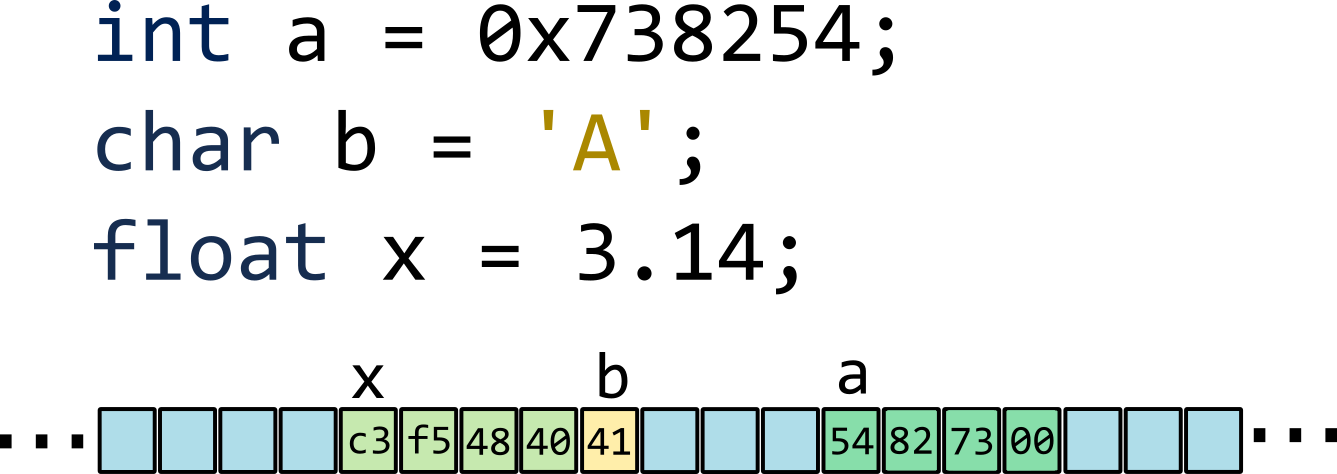
\includegraphics[scale=1]{../images/memory/memory_2_different_types.png}
\end{center}
Какие выводы можно сделать из этого изображения:
\begin{itemize}
\item Значение одного байта памяти удобно представлять двузначным шестнадцатиричным числом.
\item Каждая переменная заняла столько байт, чему равен её размер.
\item Переменные в памяти могут хранится не в том порядке, в котором вы их объявляете.
\item Переменные в памяти хранятся не обязательно вплотную друг к другу.
\item Байты переменных \texttt{a} и \texttt{b} хранятся в обратном порядке. Такой порядок байт называется \texttt{Little Endian}.  Обратите внимание, что обращается только порядок байт, а не бит. Большинство компьютеров применяют именно такой порядок байт. Но в некоторых системах может использоваться обычный порядок байт -- \texttt{Big Endian}. Обратный порядок байт применяется не только к типу \texttt{int}, но и ко всем базовым типам.
\item Переменная \texttt{b} хранит ASCII-код символа \texttt{A}. Он который равен $65 = 41_{16}$.
\end{itemize}


\newpage
\section*{Указатели разных типов}
Как вы могли заметить тип указателя зависит от типа элемента на который он указывает. Но все указатели, независимо от типа, по сути хранят одно и то же (адрес первого байта переменной). Чем же они различаются друг от друга? Разница проявляется как раз при их разыменовывании . Например, при разыменовывании указатель \texttt{int*} берёт 4 байта и воспринимает их как переменную типа \texttt{int}, а указатель \texttt{char*} берёт 1 байт и воспринимает его как переменную типа \texttt{char}.\\

Рассмотрим следующий пример. На переменную \texttt{a} указывают две переменные разных типов: \texttt{int*} и \texttt{char*}. Оба указателя хранят одно и то же значение, но работают по разному при разыменовании.

\begin{multicols}{2}
\begin{lstlisting}
#include <stdio.h>
int main() 
{
    int a = 0x12345678;
    int* p = &a;
    char* q = &a;
    
    printf("%p %p\n", p, q);
    printf("%x\n", *p);
    printf("%x\n", *q);
}
\end{lstlisting}
\vfill
\columnbreak
\hfill \break
\begin{center}
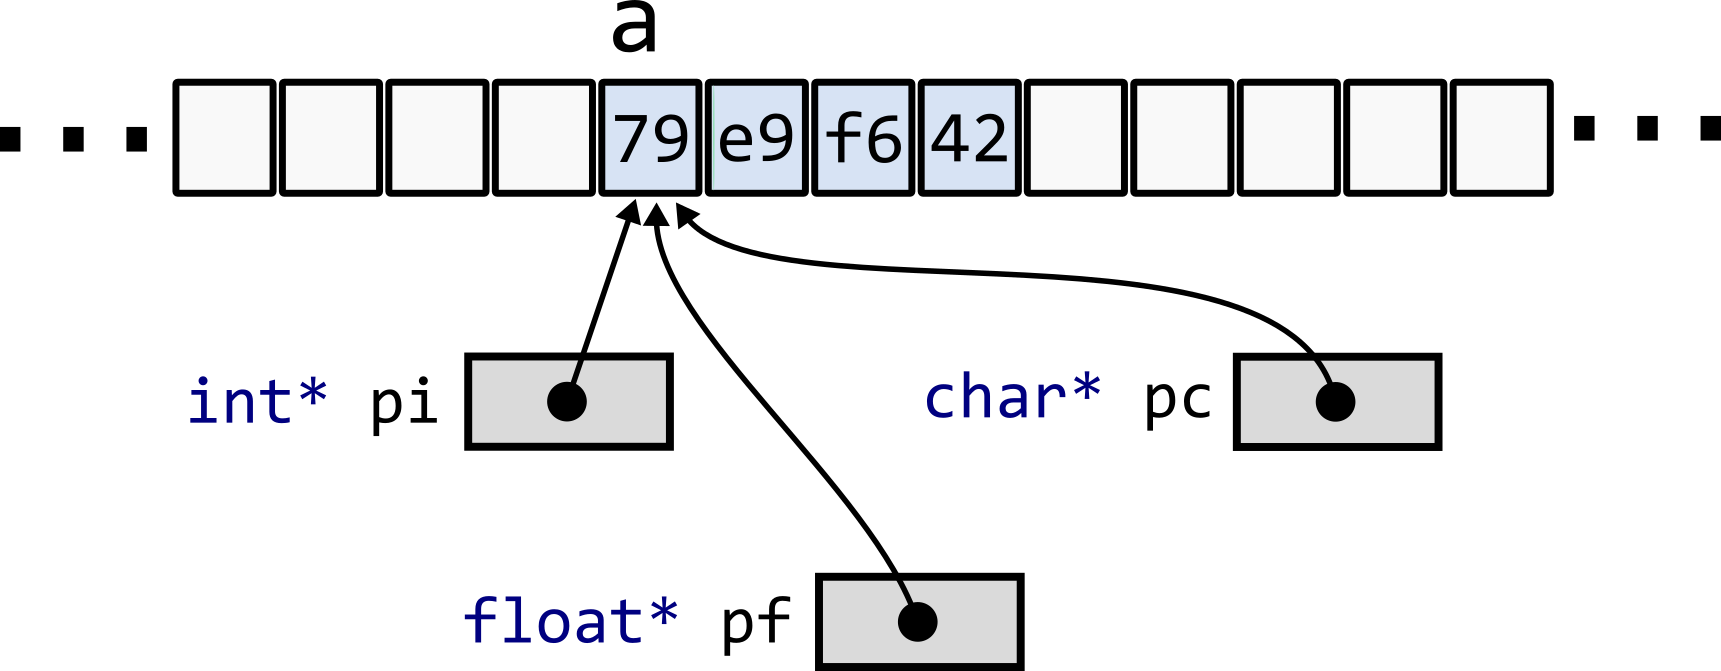
\includegraphics[scale=0.65]{../images/memory_int_char_pointer.png}
\end{center}
\hfill \break
\end{multicols}


\subsection*{Преобразование типов указателя}
В предыдущем примере есть такая строка \texttt{char* p = \&a;} Необычность этой строки в том, что слева и справа от знака \texttt{=} находятся объекты разных типов. Слева -- \texttt{char*}, а справа -- \texttt{int*}. В этот момент происходит неявное преобразование типов один тип указателя преобразуется в другой. Это всё похоже на преобразование типов обычных переменных.
\begin{lstlisting}
int a = 4.1;         // Неявное преобразование из double в int
int b = (int)4.1;    // Явное преобразование из double в int

char* p = &a;        // Неявное преобразование из int* в char*  ( не работает в C++ )
char* p = (char*)&a; // Явное преобразование  из int* в char*
\end{lstlisting}
Надо отметить, что язык \texttt{C++} строже относится к соблюдению типов, чем язык \texttt{C}, и не позволит вам неявно преобразовать указатель одного типа в указатель другого типа.

\subsubsection*{Задача: Что напечатает следующая программа и почему она это напечатает?}
\begin{lstlisting} 
#include <stdio.h>
int main() 
{
    int a = 7627075;
    char* p = (char*)&a;
    printf("%s\n", p);
}
\end{lstlisting}



\newpage
\section*{Часть 2: Просмотр байт}
\subsection*{Просмотр байт переменной}
Просмотреть, что содержится в байтах какого-либо объекта можно с помощью указателя на \texttt{unsigned char}.

\begin{lstlisting} 
#include <stdio.h>
int main() 
{
    int a = 0x11223344;
    
    unsigned char* p = (unsigned char*)&a;
    for (size_t i = 0; i < sizeof(a); ++i)
        printf("%x ", *(p + i));
    printf("\n");
}
\end{lstlisting}

\subsubsection*{Задача:}

\begin{itemize}
\item Напечатайте байты объекта \texttt{a} типа \texttt{double}.
\begin{lstlisting} 
double a = 123.456;
\end{lstlisting}

\item Напечатайте байты объекта \texttt{b} типа \texttt{int}.
\begin{lstlisting} 
int b = -1;
\end{lstlisting}

\item Напечатайте байты объекта \texttt{c} типа \texttt{struct cat}.
\begin{lstlisting} 
struct cat
{
    char first;
    int second;
};

int main()
{
    struct cat c = {0x50, 0x12345678}
}

\end{lstlisting}


\end{itemize}



\section*{Часть 3: Работа с памятью. Стандартные функции \texttt{memset}, \texttt{memcpy} и \texttt{memmove}.}




\newpage
\section*{Часть 4: Работы с бинарными файлами \texttt{fread} и \texttt{fwrite}}
\texttt{fwrite} записывает некоторый участок памяти в файл без обработки. \\
\texttt{fread} считывает данные из файла в память без обработки.

Пример. Записываем 4 байта памяти переменной \texttt{a} в файл \texttt{binary.dat}:
\begin{lstlisting}
#include <stdio.h>
int main() 
{
    int a = 0x11223344;
    FILE* fb = fopen("binary.dat", "wb");
    fwrite(&a, sizeof(int), 1, fb);
    fclose(fb);
}
\end{lstlisting}

\begin{itemize}
\item \textbf{Печать в текстовом и бинарном виде:}\\
В файле \texttt{text\_and\_binary.c} содержится пример записи числа в текстовом и бинарном виде. Скомпилируйте эту программу и запустите. Должно появиться 2 файла (\texttt{number.txt} и \texttt{number.bin}). Изучите оба эти файла, открывая их в текстовом редакторе, а также с помощью утилиты \texttt{xxd}. Объясните результат.


\item \textbf{Печать массива в бинарном виде:}\\
Пусть есть массив из чисел типа \texttt{int}: \texttt{int array[5] = \{111, 222, 333, 444, 555\};}\\
Запишите эти числа в текстовый файл \texttt{array.txt}, используя \texttt{fprintf}. Изучите содержимое этого файла побайтово с помощью \texttt{xxd}.\\
Запишите эти числа в бинарный файл \texttt{array.bin}, используя \texttt{fwrite}. Изучите содержимое этого файла побайтово с помощью \texttt{xxd}.
\end{itemize}


\newpage
\section*{Часть 5: Работа с файлами. Функции \texttt{fgetc}, \texttt{fseek}, \texttt{ftell}.}
\subsection*{Функция \texttt{fgetс}.}
Функция \texttt{fgetc} считывает 1 символ и возвращает код \texttt{ASCII} символа или \texttt{EOF} если дошли до конца файла (\texttt{EOF} это просто константа равная -1). Пример считывания:

\begin{lstlisting}
#include <stdio.h>
int main()
{
    FILE* f = fopen("test.txt", "r");
    while (1)
    {
        // Считываем 1 символ
        int c = fgetc(f);
		
        // Если он равен EOF, то выходим из цикла
        if (c == EOF)
            break;
            
        printf("%c\n", c);
	}
    fclose(f);
}
\end{lstlisting}

\begin{itemize}
\item Напишите программу, которая печатает количество строк в файле.
\item Напишите программу, которая печатает размер самой длинной строки файла.
\end{itemize}


\subsection*{Функции \texttt{ftell} и \texttt{fseek}.}
Процесс считывания файла можно представить как перемещение по набору байт. При открытии файла указатель положения равен нулю. При считывании он увеличивается на количество считанных байт.
\begin{center}
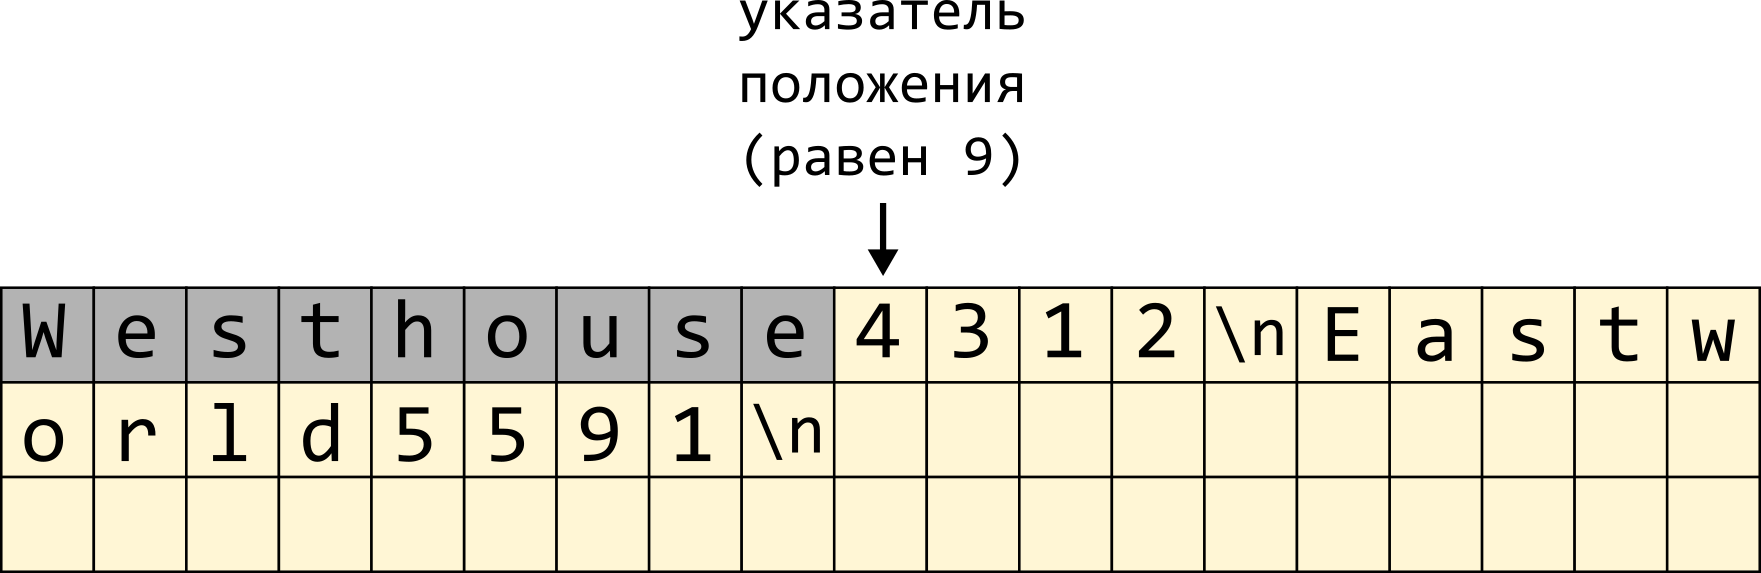
\includegraphics[scale=0.8]{../images/positioninfile.png}
\end{center}

Однако, положение в файле можно менять и без считывания при помощь функции \texttt{fseek}:
\begin{verbatim}
fseek(<файловый указатель>, <смещение>, <начало отсчёта>)
\end{verbatim}
Начало отсчёта в этой функции может принимать 3 значения:
\begin{enumerate}
\item \texttt{SEEK\_SET} -- отсчитывать от начала файла
\item \texttt{SEEK\_CUR} -- отсчитывать от текущего положения
\item \texttt{SEEK\_END} -- отсчитывать от конца файла
\end{enumerate}

Например:
\begin{lstlisting}
#include <stdio.h>
int main()
{
    FILE* f = fopen("test.txt", "r");
    fseek(f, 10, SEEK_SET); // Перемещаемся на 11 - й символ
    fseek(f, -1, SEEK_END); // Перемещаемся к последнему символу
	
    fseek(f, -1, SEEK_CUR); // Перемещаемся на 1 символ назад
    fseek(f, 0, SEEK_SET);  // Возвращаемся к началу
    fclose(f);
}

\end{lstlisting}

Функция \texttt{ftell(<файловый указатель>)} возвращает целое число -- текущее положение в файле.

\begin{itemize}
\item Написать программу, которая будет печатать 3 последних символа в файле.\\
\item Написать программу, которая будет считывать файл \texttt{test.txt} и печатать число, которое начинается с 10-го символа.
\item Написать программу, которая будет принимать название файла через аргумент командной строки и печатать его размер в байтах.\\
\textit{Подсказка:} Используйте \texttt{fseek}, чтобы перейти в конец файла и \texttt{ftell}, чтобы узнать позицию.

\item В файле \texttt{numbers.txt} хранятся некоторые целые числа (но не указано их количество). Напишите программу, которая будет считывать все числа из этого файла и печатать их на экран. Есла в файле содержится какие-то другие символы кроме цифр и пробельных символов, то программа должна печатать \texttt{Error!} и завершаться.\\
\textit{Подсказка:} Для начала нужно узнать количество чисел. Это можно сделать, используя \texttt{fgetc}. Затем считываем. Память для чисел выделяем в куче, так как их количество изначально неизвестно и может быть болишим.
\end{itemize}






\newpage
\section*{Часть 6: Работа с изображениями формата \texttt{.ppm}}
Простейший формат для изображение имеет следующую структуру
\begin{verbatim}
P3
3 2
255
255 0 0 
0 255 0  
0 0 255 
255 255 0 
255 255 255 
0 0 0
\end{verbatim}
\begin{itemize}
\item В первой строке задаётся тип файла \texttt{P3} - означает, что в этом файле будет храниться цветное изображение, причём значения пикселей будет задаваться в текстовом формате.
\item Во второй строке задаются размеры картинки - 3 на 2 пикселя.
\item Во третьей строке задаётся максимальное значение RGB компоненты цвета.
\item Дальше идут RGB компоненты цветов каждого пикселя в текстовом формате.
\end{itemize}
Картинка имеет следующий вид:
\begin{center}

\includegraphics[scale=0.5]{../images/tiny.png}
\end{center}

\subsection*{Задачи}
\begin{itemize}
\item Написать программу, которая генерирует одноцветную картинку (500 на 500) в формате \texttt{.ppm}. Цвет должен передаваться через аргументы командной строки.
\item \textbf{Белый шум:} Написать программу, которая случайное изображение в формате \texttt{.ppm}. Цвет каждого пикселя задаётся случайно.
\item \textbf{Градиент:} Написать программу, которая генерирует градиентную картинку в формате \texttt{.ppm}. Два цвета должны передаваться через аргументы командной строки.
\item \textbf{Черно-белая картинка:} Написать программу, которая считывает изображение в формате \texttt{.ppm} и сохраняет его в черно-белом виде. Файл изображения должен передаваться через аргументы командной строки. Считайте файл \texttt{russian\_peasants\_1909.ppm} и сделайте его черно-белым.
\end{itemize}


\newpage
\section*{Часть 4: Работа с изображениями формата \texttt{.jpeg}}




\end{document}